\documentclass{beamer}
\usetheme{Frankfurt}

\usepackage[utf8]{inputenc}
\usepackage{amssymb}
\usepackage{physics}

\setbeamertemplate{navigation symbols}{}

\DeclareMathOperator{\id}{id}
\DeclareMathOperator{\Span}{span}

\title{Quantum Logic}
\subtitle{A logic based approach to Bell's inequalities\cite{Burbano2017}}
\author[Iván Burbano]{Iván Mauricio Burbano Aldana}
\institute{Universidad de los Andes}
\date{\today}

\begin{document}

\begin{frame}

	\titlepage

\end{frame}

\begin{frame}

	\frametitle{Outline}
	\tableofcontents

\end{frame}

\section{EPR Paradox}

\begin{frame}

	\frametitle{Completeness of Quantum Mechanics}
	
	Einstein, Podolsy and Rosen, although weary of the success of quantum mechanics, wanted to probe its completeness\cite{Einstein1935}.
	
	\begin{itemize}
		
		\item In a complete physical theory every element of physical reality has a counterpart in the theory.		
		
		\item If we can predict with certainty the value of a physical cuantity without disturbing the system, then there exists an element of physical reality corresponding to this physical quantity.
		
	\end{itemize}

\end{frame}

\begin{frame}

	\frametitle{Let's Put It to the Test}

	Well, as we've learned from our mathematician friends, lets assume it is!
	
	\begin{block}{Heisenberg's Uncertainty Principle}

		If two observables are represented by operators which do not commute they cannot be measured simultaneously, i.e., they do not have a simultaneous physical reality\cite{Hall2013}.

	\end{block}	

\end{frame}

\begin{frame}

	\frametitle{Photon Polarization}

	As an example consider the linear polarization of a photon.
	
	\begin{itemize}
	
		\item Hilbert space $\mathbb{C}^2$;
		\item Vector state describing polarization along the angle $\theta$ 
		\begin{equation}
			\ket{\theta}=(\cos(\theta),\sin(\theta));
		\end{equation}
		\item Operator describing ``The polarization of the photon is along $\theta$''
		\begin{equation}
			P(\theta)=\dyad{\theta}.
		\end{equation}
	
	\end{itemize}

\end{frame}

\begin{frame}

	\frametitle{Two Photons}
	
	\begin{figure}
		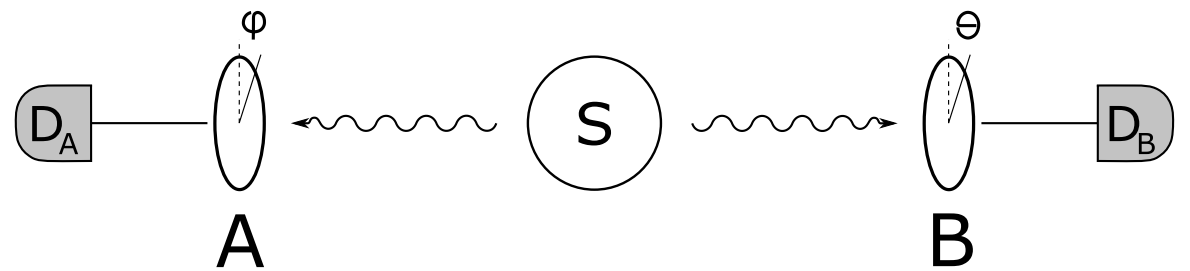
\includegraphics[width=0.7\textwidth]{bell_experiment.png}
	\end{figure}		
	
	We emmit two photons in the state
	\begin{align}
	\begin{split}
		\ket{\psi}=&\frac{1}{\sqrt{2}}(\ket{0}\otimes\ket{\pi/2}-\ket{\pi/2}\otimes\ket{0})\\
		=&\frac{1}{\sqrt{2}}(\ket{\pi/4}\otimes\ket{3\pi/4}-\ket{3\pi/4}\otimes\ket{\pi/4})\in\mathbb{C}^2\otimes\mathbb{C}^2.
	\end{split}
	\end{align}
	Alice measures the first component $P_A(\varphi)=P(\varphi)\otimes\id_{\mathbb{C}^2}$ and Bob the second $P_B(\theta)=\id_{\mathbb{C}^2}\otimes P(\theta)$. Such a state can be prepared through the decay of a Calcium atom\cite{Reyes2013}.

\end{frame}

\begin{frame}

	\frametitle{Contradiction!}
	
	Through Bob's measurements we may acquire information of Alice's system due to the process known as collapse of the wave function. Indeed, if Bob measures $P_B(0)$ then we can predict what the result of Alice's $P_A(0)$ measurement will be. Since Bob's measurements cannot affect Alice's system $P_A(0)$ becomes and element of physical reality. The same is true for $P_B(\pi/4)$ and $P_A(\pi/4)$. Thus $P_A(0)$ and $P_A(\pi/4)$ both have a simultaneous reality! Since $[P_A(0),P_A(\pi/4)]\neq 0$ we've arrived to a contradiction. 

\end{frame}

\section{Bell's Inequalities}

\begin{frame}

	\frametitle{The Search for a Complete Theory}
	
	Under the definitions given by EPR quantum mechanics is not complete. Can we provide a complete theory of physical reality? Bell while studying this question arrived at his inequalities for a theory of hidden variables\cite{Bell1964}. Our approach will be quite different.

\end{frame}
	
\begin{frame}

	\frametitle{Partially Ordered Sets}
	
	\begin{definition}
	
		A partially ordered set (poset) $(P,\leq)$ is a set $P$ along with a relation $\leq$ which is:
		\begin{itemize}
		
			\item reflexive: $p\leq p$ for all $p\in P$;
			\item anti-symmetric: $p\leq q$ and $q\leq p$ implies $p=q$ for all $p,q\in P$;
			\item transitive: $p\leq q$ and $q\leq r$ implies $p\leq r$ for all $p,q,r\in P$.   		
		
		\end{itemize}			
	
	\end{definition}
	
	\begin{example}	
	
		\begin{itemize}
	
			\item $(\mathbb{R},\leq)$
			\item $(P(X),\subseteq)$
			\item $(\text{Propositions},\Rightarrow)$!	
	
		\end{itemize}
	
	\end{example}

\end{frame}	

\begin{frame}

	\frametitle{Meet and Join}
	
	\begin{definition}
	
		Let $(P,\leq)$ be a poset and $p,q\in P$. We define $p\wedge q$ to be the greatest least bound of $\{p,q\}$ if it exists. Similarly $p\vee q$ is the lowest upper bound of $\{p,q\}$ if it exists.	If for every pair $p,q\in P$ both $p\wedge q$ and $p\vee q$ exist the poset is said to be a lattice.
	
	\end{definition}

	Notice that this definition can easily be extended to subsets with more than two elements.

	\begin{definition}
		
		A poset $(P,\leq)$ is said to be bounded if there is a greatest lower bound $0$ and a least upper bound $1$. A complement of $p\in P$ is an element $q\in P$ such that $p\wedge q=0$ and $p\vee q=1$		
		
	\end{definition}

\end{frame}

\begin{frame}

	\frametitle{Examples of Meets and Joins}
	
	\begin{example}
	
		\begin{itemize}
		
			\item $(\mathbb{R},\leq)$ is an unbounded lattice where $x\wedge y=\min\{x,y\}$ and $x\vee y=\max\{x,y\}$.
		
			\item $(P(X),\subseteq)$ is a bounded lattice where $A\wedge B=A\cap B$, $A\vee B=A\cup B$, $0=\emptyset=A\cap A^c$, and $1=X=A\cup A^c$.
			
			\begin{figure}
			\includegraphics[width=0.3\textwidth]{intersection_of_sets_A_and_B.png}
			\end{figure}		
			
			\item $(\text{Propositions},\Rightarrow)$ form a bounded lattice where $p\wedge q$ is the conjunction of the propositions, $p\vee q$ is the disjunction, $0$ is always true, and $1$ is always false. The complement of $p$ is its negation $\neg p$.
		
		\end{itemize}			
	
	\end{example}

\end{frame}

\begin{frame}

	\frametitle{Distributivity}

	\begin{definition}
	
		A lattice $(L,\leq)$ is said to be distributive if $p\wedge(q\vee r)=(p\wedge q)\vee(p\wedge r)$ and $p\vee (q\wedge r)=(p\vee q)\wedge (p\vee r)$ for all $p,q,r\in L$.	
	
	\end{definition}
	
	\center
	\begin{tabular}{|c|c|c|c|c|c|c|c|}
	\hline
	$p$ & $q$ & $r$ & $q\vee r$ & $p\wedge q$ & $p\wedge r$ & $p\wedge(q\vee r)$ & $(p\vee q)\wedge(p\vee r)$ \\
	\hline
	T & T & T & T & T & T & T & T \\
	T & T & F & T & T & F & T & T \\
	T & F & T & T & F & T & T & T \\
	T & F & F & F & F & F & F & F \\
	F & T & T & T & F & F & F & F \\
	F & T & F & T & F & F & F & F \\
	F & F & T & T & F & F & F & F \\
	F & F & F & F & F & F & F & F \\
	\hline
	\end{tabular}

\end{frame}

\begin{frame}

	\frametitle{Boolean Algebras}
	
	\begin{definition}
	
		A Boolean algebra is a distributive bounded lattice in which every element has a complement.	
	
	\end{definition}

	One can prove that in these algebras the complement is unique. Therefore, the complement of $p$ in a Boolean algebra will be denoted by $p'$.

	\begin{alertblock}{Interpretation}
		We will interpret EPR's requirements of a complete physical theory to be that the set of propositions one may ask of the theory be a Boolean algebra.
	\end{alertblock}

\end{frame}

\begin{frame}

	\frametitle{Bell's Inequalities I}
	
	Let $(B,\leq)$ be a Boolean algebra. Define
	\begin{align}
	\begin{split}
		f:B\times B&\rightarrow B\\
		(p,q)&\mapsto f(p,q):=(p\wedge q)\vee(p'\wedge q').
	\end{split}
	\end{align}
	Note that for all $p_1,q_1,p_2,q_2\in B$
	\begin{align}
	\begin{split}
		(p_1\wedge q_1)\wedge((p_1\wedge q_2)\vee(p_2'\wedge q_2')\vee(p_2\wedge q_1))=&\\
		(p_1\wedge q_1\wedge q_2)\vee(p_1\wedge q_1\wedge (p_2\vee q_2)')\vee(p_1\wedge q_1\wedge p_2)=&\\
		(p_1\wedge q_1)\wedge(q_2\vee(p_2\vee q_2)'\vee p_2)=(p_1\wedge q_1)\wedge 1=p_1\wedge q_1.&
	\end{split}
	\end{align}

\end{frame}
	
\begin{frame}
	
	\frametitle{Bell's Inequalities II}
	
	We conclude
	\begin{equation}
		p_1\wedge q_1\leq(p_1\wedge q_2)\vee(p_2'\wedge q_2')\vee(p_2\wedge q_1). 
	\end{equation}	
	Similarly
	\begin{equation}
		p_1'\wedge q_1'\leq(p_1'\wedge q_2')\vee(p_2\wedge q_2)\vee(p_2'\wedge q_1').
	\end{equation}
	Therefore
	\begin{equation}
		f(p_1,q_1)\leq f(p_1,q_2)\vee f(p_2,q_2)\vee f(p_2,q_1).
	\end{equation}	 
	
\end{frame}		

\begin{frame}

	\frametitle{Bell's Inequalities III: Degrees of Plausibility}
	
	In quantum mechanics we are more comfortable with the assignment of probabilities to propositions\cite{Jaynes2003}. Any reasonable assignment $P:B\rightarrow \mathbb{R}$ of degree of plausibility to physical propositions must be such that $P(p)\leq P(q)$ if $p\leq q$. Moreover, $P(p\vee q)\leq P(p)+P(q)$. We thus arrive at

	\begin{theorem}[Bell's Inequalities]
	
		Let $(B,\leq)$ be a Boolean algebra with an assignation of degrees of plausibility $P$. Then
		\begin{equation}
			P(f(p_1,q_1))\leq P(f(p_1,q_2))+P(f(p_2,q_2))+P(f(p_2,q_1)).
		\end{equation}			
	
	\end{theorem}

\end{frame}

\section{Lattice of Propositions in Quantum Mechanics}

\begin{frame}

	\frametitle{What are Propositions in Quantum Mechanics?}
	
	Propositions in quantum mechanics should be observables with only two possible values when measured: True or False\cite{Wilce2012}.
	
	\begin{itemize}
	
		\item Observable $\rightarrow$ Self-adjoint operator
		
		\item Spectrum $\{\text{False},\text{True}\}\rightarrow\{0,1\}$	
	
	\end{itemize}
	
	\begin{definition}
	
		We define propositions in quantum mechanics to be the orthogonal projections $L(\mathcal{H}):=\{P\in\mathcal{B}(\mathcal{H})|P^2=P=P^*\}$.	
	
	\end{definition}

\end{frame}
	
\begin{frame}

	\frametitle{Geometry on Hilbert Spaces}
	
	Once again, much like mathematicians, given that it is not clear how to define a poset structure on $L(\mathcal{H})$ we have to proceed by duality.
	
	\begin{theorem}
	
		Every closed subspace of $\mathcal{H}$ is the image of an orthogonal projection. Conversely, the image of every orthogonal projection is a closed subspace of $\mathcal{H}$.	
	
	\end{theorem}
	
	We may thus understand $L(\mathcal{H})$ as the set of closed subspaces of $\mathcal{H}$.

\end{frame}	

\begin{frame}

	\frametitle{Partial Order on $L(\mathcal{H})$}
	
	We inherit the Poset structure from $P(\mathcal{H})$. 
	
	\begin{definition}
	
		The poset of propositions in quantum mechanics is $(L(\mathcal{H}),\subseteq)$.	
	
	\end{definition}

This forms a bounded lattice:

	\begin{itemize}
	
		\item $P\wedge Q=P\cap Q$;
		\item $P\vee Q = \overline{\Span (P\cup Q)}$;
		\item $0=\{0\}$;
		\item $1=\mathcal{H}$.
	
	\end{itemize}
	
	\begin{theorem}
		
		If $P,Q\in L(\mathcal{H})$ commute $P\wedge Q=PQ$ and $P\vee Q=P+Q-PQ$.		
		
	\end{theorem}

\end{frame}

\begin{frame}

	\frametitle{Degrees of Plausibility in Quantum Mechanics}
	
	In quantum mechanics every state determines a degree of plausibility on $L(\mathcal{H}),\subseteq)$. In particular, vector states $\ket{\psi}\in\mathcal{H}$ determine the degree of plausibility
	\begin{equation}
		P_\psi(P)=\ev{P}{\psi}.
	\end{equation}
	One verifies that if $P\leq Q$ then
	\begin{align}
	\begin{split}
		\|P\ket{\psi}\|^2=&\ev{P^2}{\psi}=\ev{P}{\psi}=P_\psi(P)=P(PQ)\\
		=&\ev{PQ}{\psi}\leq\|P\ket{\psi}\|\|Q\ket{\psi}\|\leq\|Q\ket{\psi}\|^2\\
		=&P_\psi(Q).
	\end{split}
	\end{align}
	Moreover, one can check that
	\begin{equation}
		P_\psi(P\vee Q)\leq P_\psi(P)+P_\psi(Q).
	\end{equation}

\end{frame}

\begin{frame}

	\frametitle{Back to EPR}
	
	Notice that $[P_A(\theta),P_B(\phi)]=0$. Thus the proposition we assign to their conjunction ``Alice measures polarization at an angle $\theta$ while Bob at an angle $\phi$'' is $P_A(\theta)\wedge P_B(\phi)=P_A(\theta)P_B(\phi)=P(\theta)\otimes P(\phi)$. The expected values are
	\begin{align}
	\begin{split}
		P(P_A(\theta)\wedge P_B(\phi))=\ev{P_A(\theta)P_B(\phi)}{\psi}&=\\
		\frac{1}{\sqrt{2}}\bra{\psi}\qty(P(\theta)\ket{0}\otimes P(\phi)\ket{\pi/2}-P(\theta)\ket{\pi/2}\otimes P(\phi)\ket{0})&=\\
		\frac{1}{\sqrt{2}}\bra{\psi}\qty(\cos(\theta)\ket{\theta}\otimes \sin(\phi)\ket{\phi}-\sin(\theta)\ket{\theta}\otimes\cos(\phi)\ket{\phi})&=\\
		\frac{1}{2}\qty(\cos(\theta)\sin(\phi)-\sin(\theta)\cos(\phi))^2&=\\
		\frac{1}{2}\sin(\theta-\phi)^2.&
	\end{split}
	\end{align}

\end{frame}

\begin{frame}

	\frametitle{Coincidences in Quantum Mechanics}
	
	It makes sense to choose as complements $P_A(\theta)'=P_A(\theta+\pi/2)$ and $P_B(\theta)'=P_B(\theta+\pi/2)$. It is clear then that 
	\begin{equation}
		P(P_A(\theta)'\wedge P_B(\phi)')=\frac{1}{2}\sin(\theta-\phi)^2.
	\end{equation}
	On the other hand, notice that
	\begin{align}
	\begin{split}
		(P_A(\theta)'\wedge P_B(\phi)')(P_A(\theta)\wedge P_B(\phi))&=\\
		P_A(\theta+\pi/2)P_B(\phi+\pi/2)P_A(\theta)P_B(\phi)&=\\
		(P(\theta+\pi/2)\otimes P(\phi+\pi/2))(P(\theta)\otimes P(\phi)))&=\\
		P(\theta+\pi/2)P(\theta)\otimes P(\phi+\pi/2)P(\phi)&=\\
		0=(P_A(\theta)\wedge P_B(\phi))(P_A(\theta)'\wedge P_B(\phi)')&.
	\end{split}
	\end{align}	 
	Thus, we obtain
	\begin{align}
	\begin{split}
	f(P_A(\theta),P_B(\phi))=&(P_A(\theta)\wedge P_B(\phi))\vee(P_A(\theta)'\wedge P_B(\phi)')\\
	=&P_A(\theta)\wedge P_B(\phi)+P_A(\theta)'\wedge P_B(\phi)'.
	\end{split}
	\end{align}

\end{frame}

\begin{frame}

	\frametitle{Violations of Bell's Inequalities}

	Since expected values are linear, 
	\begin{equation}
	P(f(P_A(\theta),P_B(\phi)))=\sin(\theta-\phi)^2.
	\end{equation}
	
	Thus Bell's inequalities dictate	
	\begin{align}
	\begin{split}
	1=&\sin(0-\pi/2)^2=P(f(P_A(0),P_B(\pi/2)))\\
	\leq&\sin(0-\pi/6)^2+\sin(\pi/3-\pi/6)^2+\sin(\pi/3-\pi/2)^2\\
	=&3/4.
	\end{split}
	\end{align}

\end{frame}

\begin{frame}

	\frametitle{Conclusion}
	
	\Huge There is no correct physical theory whose propositions satisfy a Boolean algebra.

\end{frame}

\begin{frame}

	\frametitle{What failed?}
	
	\begin{theorem}
		
		In a distributive bounded lattice elements have at most one complement.		
		
	\end{theorem}
	
	\begin{proof}
	
		Suppose $q$ and $r$ are complements of $p$ in a distributive bounded lattice. Then
		\begin{equation}
			q=q\wedge 1=q\wedge(p\vee r)=(q\wedge p)\vee(q\wedge r)=0\vee(q\wedge r)=q\wedge r.
		\end{equation}			
		This $q\leq r$. Similarly one can show $r\leq q$. By anti-symmetry $q=r$.
	\end{proof}

It is clear that in the bounded lattice $L(\mathcal{H})$ complements are not unique. Thus the lattice is not distributive.

\end{frame}
	
\begin{frame}[allowframebreaks]
	
	\frametitle{References}

	\bibliography{../Mendeley/library}
	\bibliographystyle{apalike}

\end{frame}

\end{document}